\documentclass[12pt]{article}
\usepackage[margin=0.75in]{geometry}
\usepackage{graphicx}
\usepackage{float}
\setlength{\parindent}{0mm}

\begin{document}

{\centering
\large Physics I: Lab 05 \par
\large Energy \par
}
\hfill \break \vspace{-4mm}

In this lab you will explore how different forms of energy govern the dynamics of a given system.

Use Interactive Physics to set up the following experiment:
%
\begin{figure}[H]
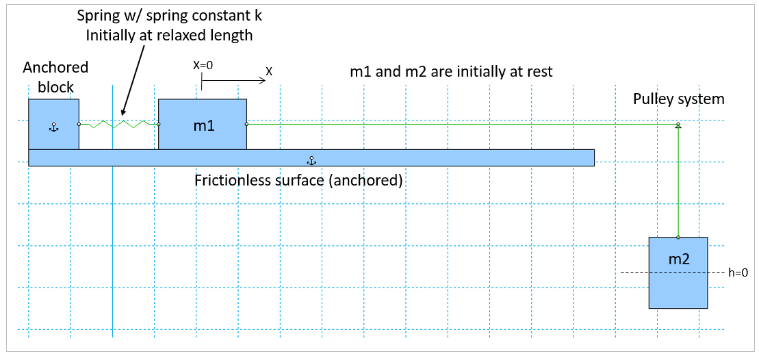
\includegraphics[scale=0.70]{figures/fig1.png}
\end{figure}
%
Note that the diagram shows a suggested coordinate system choice, but you can define your own if you prefer.
Choose some random but reasonable values for k, m1, and m2 and run the simulation and observe the results.
Before proceeding, discuss with your lab partners why you think the systems behaves the way it does (you don't need to be too quantitative yet).

\underline{\textbf{Part 1}} \par
Determine the theoretical maximum displacement of m1 with respect to its initial position.
Use the simulation to confirm your result.

\underline{\textbf{Part 2}} \par
In terms of k, m1, m2, x, v, and g, use energy conservation to write down a general equation relating these quantities at any arbitrary time t.
Choose a random value of t and use IP to find the relevant quantities at this time.
Plug these values into your equation.
Is the equation (approximately) satisfied?

\end{document}
